
% \begin{frame}{DOE ECP Acknowledgement}

% \textit{
% This research was supported by the Exascale Computing Project (17-SC-20-SC),
% a joint project of the U.S. Department of Energy’s Office of Science and National Nuclear Security Administration,
% responsible for delivering a capable exascale ecosystem, including software, applications, and hardware technology,
% to support the nation’s exascale computing imperative. 
% }

% \end{frame}

%==============================================================================

\begin{frame}{Prerequisites for Tutorial Exercises}

\textbf{Knowledge of C++}:
  class constructors, member variables, member functions, member operators, template arguments

\vspace{10pt}

% \textbf{Using NVIDIA's NVLABS}
%   \begin{itemize}
%   \item Kokkos pre installed in \$\{HOME\}/kokkos
%   \item Exercises pre installed in \$\{HOME\}/\TutorialDirectory
%   \end{itemize}

\vspace{10pt}

\textbf{Using your own {\$\{HOME\}}}
\begin{scriptsize}
  \begin{itemize}
  \item {Git}
  \item {CMake 3.16 (or newer)}
  \item {GCC 8.2 (or newer)}
    \textit{OR} {Intel 19.0.5 (or newer)}
    \textit{OR} {Clang 8.0 (or newer)}
  \item {CUDA nvcc 11.0 (or newer)}
    \textit{AND} {NVIDIA compute capability 6.0 (or newer)}
  \item {git clone \url{https://github.com/kokkos/kokkos-tutorials} \\ \hspace{2pt}  into \path{${HOME}/Kokkos/kokkos-tutorials}}
        \\ \vspace{4pt} \hspace{2pt} Slides are in \\ \hspace{8pt} \path{${HOME}/Kokkos/kokkos-tutorials/LectureSeries}
        \\ \vspace{4pt} \hspace{2pt} Exercises are in \\ \hspace{8pt} \path{${HOME}/Kokkos/kokkos-tutorials/Exercises}
  \end{itemize}
\end{scriptsize}

\end{frame}


\begin{frame}{Prerequisites for Tutorial Exercises}

\textbf{Online Resources}:

\begin{itemize}
	\item \url{https://github.com/kokkos}: Primary Kokkos GitHub Organization
	\item \url{https://kokkos.github.io/kokkos-core-wiki}: Wiki including API reference
	\item \url{https://github.com/kokkos/kokkos-tutorials}: Tutorial exercises
	\item \url{https://kokkosteam.slack.com}: Slack channel for Kokkos
\end{itemize}

\end{frame}


%==============================================================================

\begin{frame}{Lecture Series Objectives}

%  \textbf{Understand Kokkos Programming Model Abstractions}
%  \begin{itemize}
%    \item {What, how and why of \textit{performance portability}}
%    \item {Productivity and hope for future-proofing}
%  \end{itemize}

  %\pause

  \textbf{Kokkos' basic capabilities:}
  \begin{itemize}
    \item {Simple 1D data parallel computational patterns}
    \item {Deciding where code is run and where data is placed}
    \item {Managing data access patterns for performance portability}
    \item {Multidimensional data parallelism}
  \end{itemize}

  %\pause

  \textbf{Kokkos' advanced capabilities:}
  \begin{itemize}
    \item {Thread safety, thread scalability, and atomic operations}
    \item {Hierarchical patterns for maximizing parallelism}
    \item {Task based programming with Kokkos}
  \end{itemize}

  %\pause

  \textbf{Kokkos' tools and Kernels:}
  \begin{itemize}
    \item {How to profile, tune and debug Kokkos code}
    \item {Interacting with Python and Fortran}
    \item {Using Kokkos Kernels math library}
  \end{itemize}

\end{frame}

%==============================================================================

\begin{frame}{Tutorial Takeaways}

  \begin{itemize}
  \item {Kokkos enables \textbf{Single Source Performance Portable Codes}}
  \item {\textbf{Simple things stay simple} - it is not much more complicated than OpenMP}
  \item {\textbf{Advanced performance optimizing capabilities} easier to use with Kokkos than e.g. CUDA or HIP}
  \item {Kokkos provides data abstractions critical for performance portability not available in other programming models \
         \textbf{Controlling data access patterns is key for obtaining performance} }
 \item The \textbf{Kokkos Ecosystem} comes with tools (profiling, debugging, tuning, math libraries, etc.) needed for application development in professional settings
  \end{itemize}

\end{frame}

%==============================================================================

\begin{frame}{Operating assumptions (0)}

  \textbf{Assume you are here because:}
  \begin{itemize}
    \item {Want to use \textbf{all} HPC node architectures; including GPUs}
    \item {Are familiar with \textbf{C++}}
    \item {Want GPU programming to be \textbf{easier}}
    \item {Would like \textbf{portability}, as long as it doesn't hurt performance}
  \end{itemize}
  \textbf{Helpful for understanding nuances:}
  \begin{itemize}
    \item {Are familiar with \textbf{data parallelism}}
    \item {Are familiar with \textbf{OpenMP}}
    \item {Are familiar with \textbf{GPU architecture} and \textbf{CUDA}}
  \end{itemize}

\end{frame}

%==============================================================================

\begin{frame}{Operating assumptions (1)}

  \textbf{Target machine:}
  %\vspace{-10pt}
  \begin{center}
    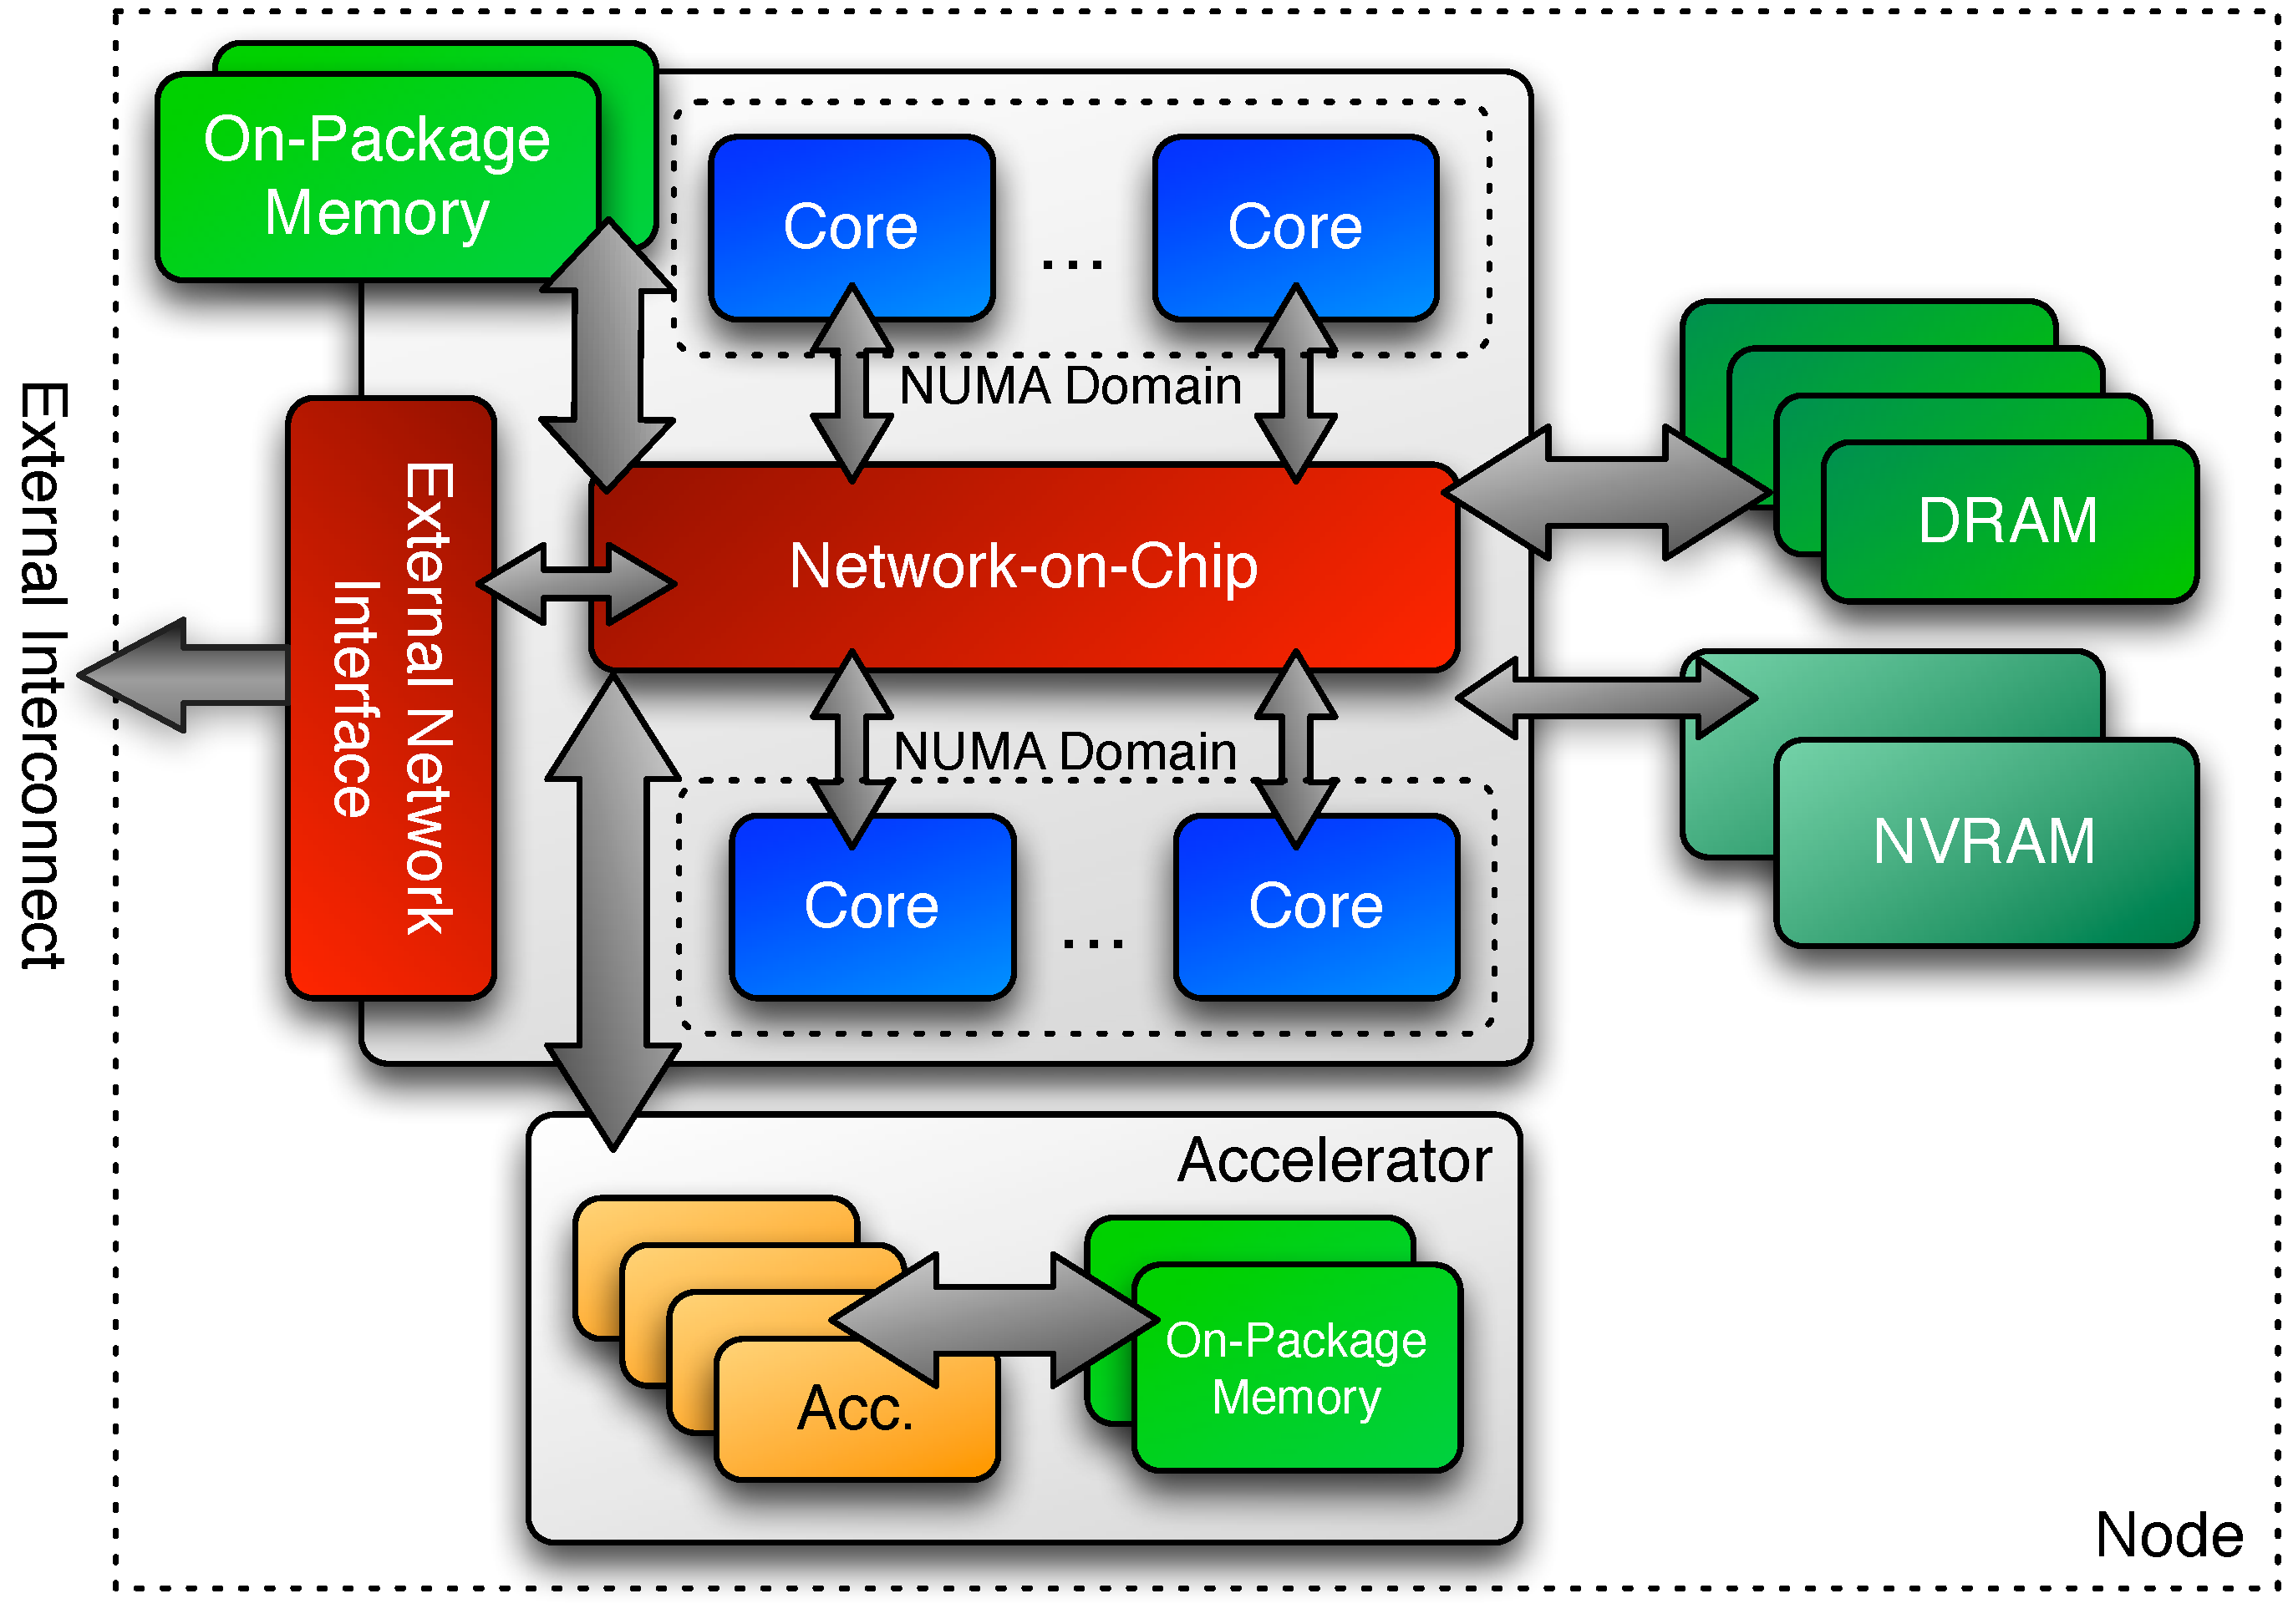
\includegraphics[width=0.80\textwidth]{figures/kokkos-node}
  \end{center}

\end{frame}

%==============================================================================

\begin{frame}[fragile]{Important Point: Performance Portability}

  \begin{block}{Important Point}
    There's a difference between \emph{portability} and
    \\ \emph{performance portability}.
  \end{block}

  \textbf{Example}: implementations may target particular architectures and may not be \emph{thread scalable}. \\
    \hspace{20pt} (e.g., locks on CPU won't scale to 100,000 threads on GPU)

  \pause
  \vspace{5pt}

  \textbf{Goal}: write \textbf{one implementation} which:
  \begin{itemize}
    \item{compiles and \textbf{runs on multiple architectures},}
    \item{obtains \textbf{performant memory access patterns} across architectures,}
    \item{can leverage \textbf{architecture-specific features} where possible.}
  \end{itemize}

  \pause
  \vspace{5pt}
  \textbf{Kokkos}: performance portability across manycore architectures.

  \vspace{5pt}

\end{frame}
